\documentclass[a4paper]{article}
\usepackage[margin=25mm]{geometry}
\usepackage[utf8]{inputenc}
\usepackage[british]{babel} 
\usepackage[parfill]{parskip} % fixes newline paragraphs
\usepackage[T1]{fontenc} % for outout char encoding to not be ascii-thingy
\usepackage[none]{hyphenat} % remove hyphenation

% Packages
\usepackage{graphicx}
\usepackage{amsmath}
\usepackage{amsfonts}
\usepackage{amssymb}
\usepackage{minted}

% Title page
\title{Hand in 3 \\ Information Theory}
\author{Fredrick Nilsson \\ fr2037ni-s}
\date{\today}

\begin{document}

\maketitle

\newpage

\section{Report}
\subsection{Part 1}

It takes 2 rounds to decode the message.

Iteration 1: 

\(\hat{v}\): 0 1 0 0 1 0 0 \\
Syndrome: 1 1 0 1 1 1 \\
\(\sigma^{(i)}\): 1 2 1 1 3 1 1 


Iteration 2: 

\(\hat{v}\): 0 1 0 0 0 0 0 \\
Syndrome: 1 1 1 0 0 0 \\
\(\sigma^{(i)}\): 1 3 2 1 1 0 0  \\

Final: 

\(\hat{v}\): 0 0 0 0 0 0 0

Resulting in the decoded message: 0 0 0 0 0 0

The code for this part is found in section \ref{sec:source12}.

The code is an implementation of the algorithm described in lecture 9. It takes a message and a parity check matrix as input, and then decodes the message using the algorithm.

\subsection{Part 2}

The decoded message is:
Life is what happens when you are busy making other plans.

The source code for this can be found in section \ref{sec:source12}.
The only thing added to the code from part 1 is the ability to scan a file for the message and parity check matrix and the translatation of the bits back to a string.

\subsection{Part 3}

For the third part I translated the provided matlab example into python, and then continued it's implementation by using a proper decoder and parity check matrix.
I also implemented a progressbar and made it multi-threaded to speed up the process.

The graph in figure \ref{fig:graph} shows the biterrors for different values of \(\epsilon\). The source code for this part can be found in section \ref{sec:source3}.
What the graph shows is that the biterrors increase as \(\epsilon\) increases. 
This is expected as the probability of a bit being flipped increases, and beyond \(\epsilon > 0.06\) the biterrors from using the algorithm is higher than the biterrors from using not having any error detection at all.
Although this is using the parity matrix given in part 2, and there might be other parity matrixes which would provide better results.

\begin{figure}[h]
    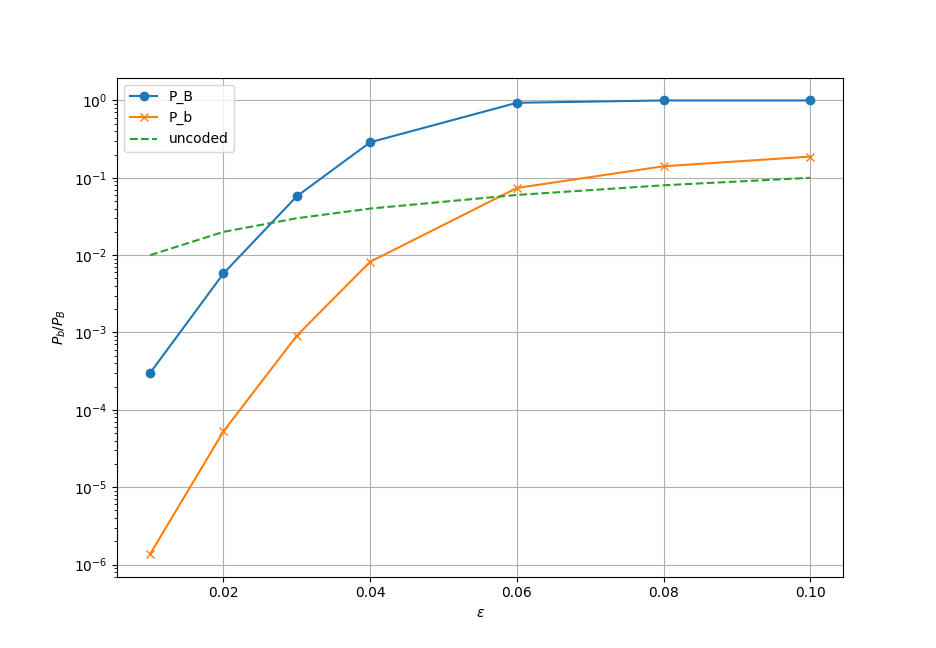
\includegraphics[width=\textwidth]{../Figure_1.png}
    \caption{Graph of the biterrors for different values of \(\epsilon\) .}
    \label{fig:graph}
\end{figure}

\newpage
\section{Source code}
\subsection{Part 1 \& 2}\label{sec:source12}
\inputminted[breaklines]{python}{../handin12.py}

\subsection{Part 3}\label{sec:source3}
\inputminted[breaklines]{python}{../handin3.py}

\end{document}
